\chapter{Teknisk beskrivelse}

\section{Databaseabstraktion}

I parallel med reservationssystemet har vi udviklet en databaseabstraktion ved navn \textit{Donkey}. Donkey er bygget oven på \textit{Java Database Connectivity} (forkortet \textit{JDBC}) og har til formål at muliggøre persistens af datamodeller uden at en udvikler behøver at skrive en eneste linje SQL. Dette opnås gennem såkaldt \textit{object-relational mapping} (forkortet \textit{ORM}), hvor et objekt i et objekt-orienteret system – i vores tilfælde Java – automatisk kan konverteres til en mere simpel struktur, som kan gemmes i et databasesystem (\cite{wiki:orm}).

Donkey understøtter på nuværende tidspunkt tre forskellige relationelle databasesystemer: MySQL\footnote{\url{http://www.mysql.com/}}, PostgreSQL\footnote{\url{http://www.postgresql.org/}}, samt SQLite\footnote{\url{http://sqlite.org/}}. Mens Bookie udelukkende gør brug af SQLite, er understøttelse af de resterende databasesystemer medtaget for at sikre en solid løsning, som kan tage forbehold for eventuelle forskelle mellem databasesystemer.

Donkeys grundlæggende byggedele er baserede på Laravels\footnote{\url{http://laravel.com/}} API'er, da disse allerede var en af forfatterne kendte. Konceptuelt låner Donkey begreberne om \textit{Grammars}, \textit{Queries}, samt \textit{Schemas} og benytter disse til at implementere ORM i form af \textit{Models}. En datamodel i Donkey er derfor i sidste ende ikke andet end en klasse, som repræsenterer en tabel i en relationsdatabase, og en række offentlige felter i denne klasse, som repræsenterer tabellens kolonner og datatyperne af disse. Dette er igen relateret til Laravel og dens \textit{Eloquent ORM}\footnote{\url{http://laravel.com/docs/4.2/eloquent}} dog med den forskel, at Donkeys implementation af ORM endnu ikke er nær så fleksibel som Laravels.

Helt konkret består Donkey af følgende klasser:

\begin{multicols}{3}
\begin{itemize}
  \item \texttt{Grammar}
    \begin{itemize}
      \item \texttt{MySqlGrammar}
      \item \texttt{PostgreSqlGrammar}
      \item \texttt{SqliteGrammar}
    \end{itemize}
  \item \texttt{Driver}
  \item \texttt{Row}
  \item \texttt{Database}
  \item \texttt{Query}
  \item \texttt{Schema}
  \item \texttt{Model}
  \item \texttt{ModelQuery}
\end{itemize}
\end{multicols}

Donkey er fra bunden opbygget efter \textit{dependency injection} designmønstret, hvor afhængigheder injiceres i afhængende klasser, frem for selv at lade de afhængende klasser finde og instantiere deres afhængigheder (\cite{wiki:di}). Dette designmønster har vi fulgt, da det gav større kontrol over, hvorledes afhængigheder flød igennem systemet. Eftersom \texttt{Grammar}-klassen er en afhængighed i næsten samtlige andre klasser (mere om dette følger), og da \texttt{Grammar} er abstrakt med de konkerete implementationer \texttt{My\-Sql\-Grammar}, \texttt{Postgre\-Sql\-Grammar}, og \texttt{Sqlite\-Grammar}, ville det have været yderst besværligt at opbygge systemet, hvis ikke denne grundlæggende afhængighed kunne injiceres i de afhængende klasser. Figur \ref{class-diagram:database-abstraction} forsøger at tydeliggøre, hvorledes de forskellige afhængigheder flyder gennem systemet, samt hvordan disse injiceres i de afhængende klasser.

\begin{figure}[h]
  \centering
  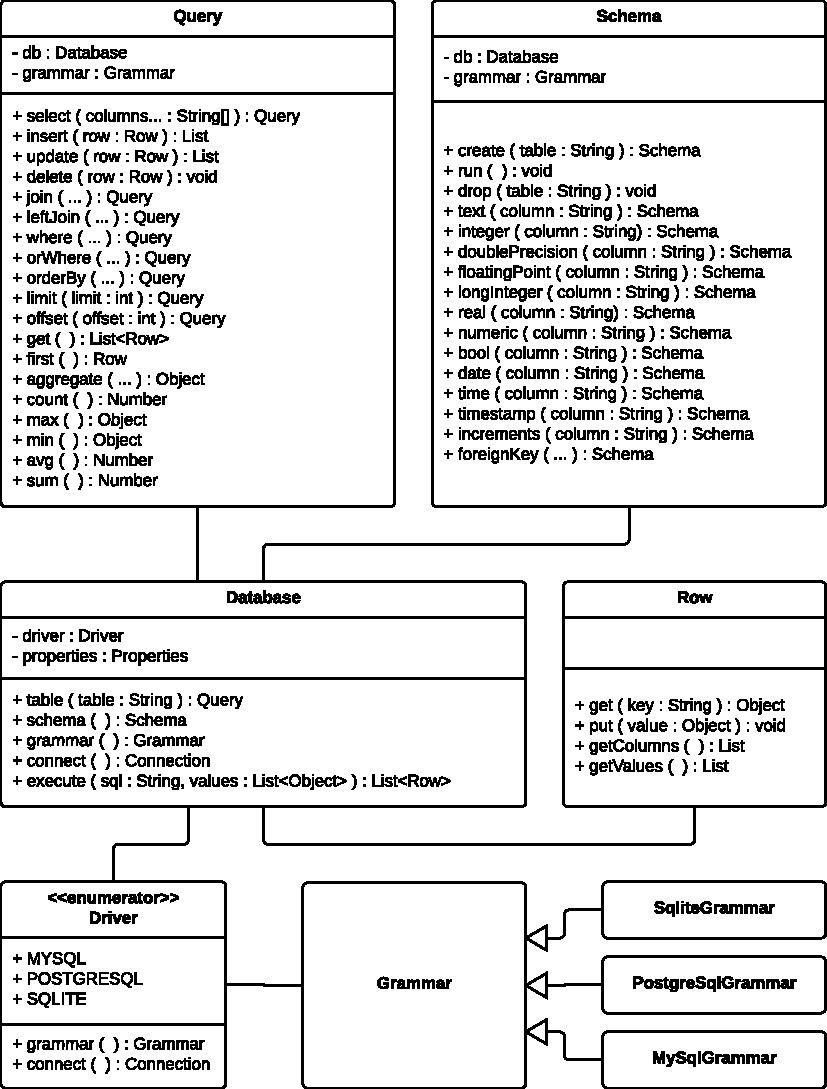
\includegraphics[scale=0.75]{database-abstraction.pdf}
  \caption{Klassediagram over databaseabstraktionen, ORM ekskluderet.}
  \label{class-diagram:database-abstraction}
\end{figure}

De næste sektioner vil gennemgå hver klasse i det niveau af detalje, som måtte være sig passende for den enkelte klasse.

\subsection{Row}

\texttt{Row}-klassen er en subklasse af \texttt{Linked\-Hash\-Map} og beskriver en datastruktur, der benyttes til at opbevare databaserækker. Den er fundamental for resten af systemet, idet den er bindeledet mellem Donkeys klasser og JDBCs \texttt{Result\-Set}\footnote{\url{https://docs.oracle.com/javase/8/docs/api/java/sql/ResultSet.html}}-strukturer, som bruges til at opbevare tabeller af data resulterende fra databaseforespørgsler.

\texttt{Row}-klassen benytter sig af de generiske typer \texttt{String} og \texttt{Object} til nøgler og værdier, respektivt, i et \texttt{Linked\-Hash\-Map}. Dette gør det muligt at associere en databasekolonne (nøglen) med en hvilken som helst datatype (værdien), hvilket er hensigtmæssigt, da en databasetabel kan indeholde mange forskellige typer af data.

Til sidst bør det nævnes, at et \texttt{Linked\-Hash\-Map} blev valgt, da iterationsrækkefølgen af kolonnerne i en tabel i visse tilfælde \textit{kan} have betydning.

\subsection{Grammar}

Den abstrakte \texttt{Grammar}-klasse benyttes til at bygge de forskellige delkomponenter af SQL-udtryk, samt til at kompilere disse delkomponenter til fulde SQL-udtryk. Som navnet på klassen indikerer, bruges den dermed til at beskrive grammatikken for SQL-udtryk:

\begin{figure}[h]
  \begin{minted}{java}
  Grammar g = new FooGrammar();

  g.addTable("table");
  g.addColumn("col1");
  g.addColumn("col2");
  g.addWhere("col1", ">", 123, "and");
  g.addWhere("col2", "=", "bar", "or");
  
  g.compileSelect();
  // => "select col1, col2 from table where col1 > ? or col2 = ?"
  \end{minted}
  \caption{Eksempel på kompilering af et \texttt{select}-udtryk via \texttt{Grammar}}
  \label{code-example:grammar-select-compilation}
\end{figure}

\begin{wrapfigure}{r}{0.35\textwidth}
  \centering
  \vspace{-12pt}
  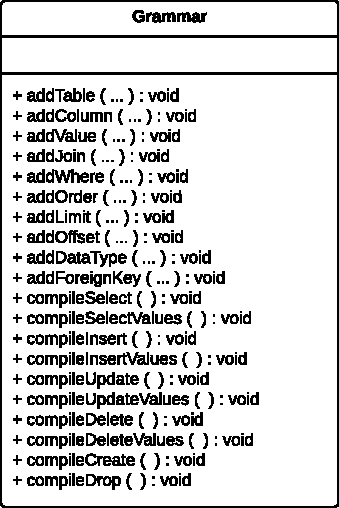
\includegraphics[width=0.275\textwidth]{grammar-class.pdf}
  \caption{Klassediagram for \texttt{Grammar}}
  \label{class-diagram:grammar-class}
\end{wrapfigure}

Læg i figur \ref{code-example:grammar-select-compilation} specielt mærke til hvorledes værdierne \texttt{123} og \texttt{"bar"} bliver erstattede med \texttt{?} i det kompilerede SQL-udtryk. Hvorfor dette gøres, vil vi komme tilbage til senere.

Målet med \texttt{Grammar}-klassen er at definere en grammatik for de mest typiske og standardiserede SQL-udtryk. Klassen er imidlertid abstrakt, da ikke alle understøttede SQL-udtryk er standardiserede mellem de forskellige databasesystemer. Dette inkluderer på nuværende tidspunkt definitionen af automatisk stigende kolonner, hvilket ikke håndteres ens mellem de understøttede databasesystemer. \texttt{Grammar} definerer derfor dette stykke funktionalitet som en abstrakt metode, der overlades til subklasser at implementere.

Figur \ref{class-diagram:grammar-class} viser de vigtigste offentlige metoder tilgængelige i \texttt{Grammar}-klassen. Alle metodeparametre er fjernede, da disse ikke umiddelbart har betydning for at danne et billede af den overordnede funktionalitet tilgængelig i \texttt{Grammar}.

\subsection{Driver}

\texttt{Driver}-enumeratoren har til opgave at oprette forbindelse til de understøttede databasesystemer via JDBCs \texttt{Driver\-Manager}\footnote{\url{http://docs.oracle.com/javase/8/docs/api/java/sql/DriverManager.html}} og de tredjepartsdrivere, som måtte være tilgængelige for det pågældende databasesystem. Derudover står \texttt{Driver}-enumeratoren også for at instantiere de konkrete \texttt{Grammar}-objekter, som skal benyttes til de forskellige databasesystemer. MySQL-driveren opretter dermed instanser af \texttt{MySql\-Grammar}, PostgreSQL-driveren instanser af \texttt{PostgreSql\-Grammar}, og til sidst SQLite-driveren instanser af \texttt{Sqlite\-Grammar}.

\texttt{Driver} er implementeret som en enumerator og ikke en klasse, da vi ikke så mening i at have et interface med tre implementerende klasser hver med kun to statiske metoder. En enumerator med to abstrakte metoder, som implementeres i hver af enumratorens elementer, var derfor at foretrække.

Der henvises til figur \ref{class-diagram:database-abstraction} for klassediagrammet for \texttt{Driver}-enumeratoren.

\subsection{Database}

\texttt{Database}-klassen står for al interaktion med de understøttede databasesystemer herunder eksekvering af SQL-forespørgsler samt tolkning af de resulterende \texttt{ResultSet}s.

Alle SQL-forespørgsler bliver eksekverede som \texttt{Prepared\-Statement}s\footnote{\url{http://docs.oracle.com/javase/8/docs/api/java/sql/PreparedStatement.html}}, og det er her, at \texttt{?}-tegnene fra de af \texttt{Grammar} kompilerede SQL-udtryk kommer ind i billedet. Et \texttt{Prepared\-Statement} bliver i første omgang sendt til SQL-serveren og pre-kompileret uden eventuelle brugergenerede parametre. Herefter indsættes de brugergenerede parametre istedet for \texttt{?}-tegnene i den pre-kompilerede forespørgsel, som herefter igen eksekveres mod serveren. Dette negerer effektivt al SQL injektion, idet SQL-serveren nu behandler de brugergenerede parametre som netop det; brugergenerede parametre. Der er derfor ikke tvivl om, at de \textit{ikke} er del af et SQL-udtryk. Ondsindet, omend gyldig SQL kan derfor indsættes som parameter, uden at det vil få indflydelse på den allerede kompilerede SQL-forespørgsel.

Ovenstående er årsagen til inklusionen af metoder som \texttt{compile\-Select\-Values()}, \texttt{compile\-Insert\-Values()}, m.v. som set i figur \ref{class-diagram:grammar-class}. Disse bliver brugt til at kompilere lister af de værdier, hvilke bliver erstattede med \texttt{?}-tegn i de kompilerede SQL-udtryk.

Til sidst står \texttt{Database} for at tolke de \texttt{Result\-Set}s, som måtte resultere fra SQL-forespørgsler. Efter hver forespørgsel gennemløbes det resulterende \texttt{Result\-Set} og oversættes til en liste af \texttt{Row}s. Forbindelsen til det pågældende \texttt{Result\-Set} kan herefter lukkes, mens indholdet – nu oversat til \texttt{Row}s – kan returneres til kalderen.

Givet et konkret \texttt{Grammar}-objekt (\texttt{g}) kan SQL eksekveres mod en server på følgende måde:

\begin{figure}[h]
  \begin{minted}{java}
  Properties config = new Properties();
  config.put(...);
  
  Database db = new Database(Driver.SOME_DRIVER, config);
  List<Row> response = db.execute(
    g.compileSelect(), g.compileSelectValues()
  );
  \end{minted}
  \caption{Eksempel på eksekvering af en SQL-forespørgsel}
  \label{code-example:sql-execution}
\end{figure}

Figur \ref{code-example:sql-execution} viser første eksempel på injektion af afhængigheder. Den ønskede \texttt{Driver} injiceres under instantieringen af \texttt{Database} sammen med eventuelle konfigurationsparametre. Dette giver os imidlertid endnu ikke nogen fordel, eftersom eksemplet gør direkte brug af en konkret \texttt{Grammar}-instans. De næste to sektioner vil dog beskrive den tilsigtede brug af \texttt{Grammar} i relation til \texttt{Database}.

\subsection{Query}

\texttt{Query}-klassen beskæftiger sig med de typer af SQL-udtryk, som under eet er kendt som \textit{Data Manipulation Language} (forkortet \textit{DML}). DML bliver brugt til at hente, indsætte, opdatere, og slette data fra databasetabeller (\cite{wiki:dml}) og indkapsler derfor de metoder i \texttt{Grammar}, som står for dette. Der henvises til figur \ref{class-diagram:database-abstraction} for en liste over disse.

\texttt{Query}-klassen instantieres ved at injicere en instans af \texttt{Database} samt navnet på den tabel, som \texttt{Query} skal eksekvere DML-udtryk mod. \texttt{Query} får fra \texttt{Database} adgang til dennes \texttt{Driver}-instans og kan herfra tilgå den specifikke \texttt{Grammar}-subklasse, som skal benyttes til det pågældende databasesystem. Det er her, som tidligere nævnt, at injicering af afhængigheder bliver uundværdligt.

\texttt{Query}-klassen kan benyttes direkte, men er tiltænkt benyttet gennem \texttt{Database}, som via dennes \texttt{table()}-metode kan instantiere nye \texttt{Query}-objekter mod den pågælende database:

\begin{figure}[h]
  \begin{minted}{java}
  List<Row> response = db.table("table")
    .select("col1", "col2")
    .where("col1", ">", 123)
    .orWhere("col2", "bar")
    .get();
  \end{minted}
  \caption{Eksempel på brug af \texttt{Query} med samme forespørgsel som set i figur \ref{code-example:grammar-select-compilation}}
  \label{code-example:query-select}
\end{figure}

\subsection{Schema}

Modsat \texttt{Query} beskæftiger \texttt{Schema} sig med de typer af SQL-udtryk, der er kendt som \textit{Data Definition Language} (forkortet \textit{DDL}). Mens DML som sagt tager sig af at hente samt manipulere data i databasetabeller, så benyttes DDL til at definere strukturen af disse (\cite{wiki:ddl}). Som var tilfældet med \texttt{Query}, instantieres \texttt{Schema} ved at injicere en instans af \texttt{Database}, hvorfra der er adgang til et \texttt{Grammar}-objekt passende til det pågældende databasesystem.

Det bør nævnes, at alle kolonner oprettet via \texttt{Schema} er påkrævede, og derfor ikke kan være \texttt{null}. Dette designvalg blev taget, da vi udelukkende så brug for påkrævede dataværdier i Bookies datamodeller.

Der henvises til figur \ref{class-diagram:database-abstraction} for de specikke \texttt{Grammar}-metoder, som \texttt{Schema} indkapsler. Disse er primært baserede på \texttt{addDataType()}-metoden i \texttt{Grammar}, der kompilerer datatypekolonner til SQL \texttt{create}-udtryk.

Ligesom \texttt{Query} er \texttt{Schema} tiltænkt brugt gennem \texttt{Database} via dennes \texttt{schema()}-metode:

\begin{figure}[h]
  \begin{minted}{java}
  db.schema()
    .create("table")
    .integer("col1")
    .text("col2")
    .run();
  \end{minted}
  \caption{Eksempel på brug af \texttt{Schema} med udgangspunkt i tabellen tilgået i figur \ref{code-example:query-select}}
  \label{code-example:schema-create}
\end{figure}

\begin{table}[h]
  \centering
  \begin{tabular}{l | l | l | l | l}

    \multicolumn{3}{l}{\textbf{Navn}: \texttt{table}} \\

    \hline

    \textbf{Kolonne} & \textbf{Påkrævet} & \textbf{Type} & \textbf{Primær nøgle} & \textbf{Fremmed nøgle} \\

    \hline

    \texttt{col1} & Ja & \texttt{integer} & Nej & Nej \\
    \texttt{col2} & Ja & \texttt{text} & Nej & Nej \\

    \hline

  \end{tabular}
  \caption{Tabellen resulterende fra forespørgslen i figur \ref{code-example:schema-create}}
\end{table}

\clearpage

\subsection{Model}

\begin{wrapfigure}{r}{0.35\textwidth}
  \centering
  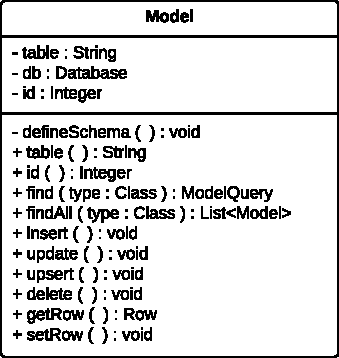
\includegraphics[width=0.275\textwidth]{model-class.pdf}
  \caption{Klassediagram for \texttt{Model}}
  \label{class-diagram:model}
\end{wrapfigure}

\texttt{Model}-klassen benytter sig af de foregående klasser til at implemenetere object-relational mapping. Dette gøres ud fra konventionen om, at subklasser af \texttt{Model} repræsenterer databasetabeller, mens subklassernes felter repræsenterer kolonnerne i disse tabeller. \texttt{Model} gør således stor brug af Javas Reflection API'er\footnote{\url{http://docs.oracle.com/javase/tutorial/reflect/}} til at hente information om de offentlige felter i en given subklasse.

\texttt{Model} benytter sig af \texttt{Schema} til at gennemløbe datamodellers offentlige felter og definere datatypekolonner for disse via \texttt{Model}s private \texttt{defineSchema()}-metode.

\texttt{Query} bliver i \texttt{Model} brugt til at indsætte, opdatere, og slette datamodeller med hjælp fra klassens \texttt{getRow()}-metode. Denne gennemløber de offentligt tilgængelige felter i en datamodel og oversætter disse til kolonner i et \texttt{Row}-objekt.

\texttt{Model} understøtter på nuværende tidspunkt en håndfuld af Javas simple typer samt disses indkapslede typer:

\begin{multicols}{3}
\begin{itemize}
  \item \texttt{String}
  \item \texttt{Integer} and \texttt{int}
  \item \texttt{Double} and \texttt{double}
  \item \texttt{Float} and \texttt{float}
  \item \texttt{Long} and \texttt{long}
  \item \texttt{Boolean} and \texttt{boolean}
\end{itemize}
\end{multicols}

Derudover er subklasser af \texttt{Model}, samt lister hvis generiske typer er subklasser af \texttt{Model}, også understøttede og benyttes til at indikere relationer datamodeller imellem.

Alle modeller indeholder kolonnen \texttt{id}, hvilken er automatisk stigende og modellens primære nøgle. Når relationer til andre datamodeller defineres, bliver dette derfor gjort via fremmede nøgler til den relaterede models \texttt{id}-kolonne.

\subsection{ModelQuery}

\begin{wrapfigure}{r}{0.35\textwidth}
  \centering
  \vspace{-12pt}
  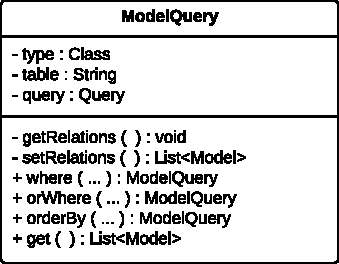
\includegraphics[width=0.275\textwidth]{modelquery-class.pdf}
  \caption{Klassediagram for \texttt{ModelQuery}}
  \label{class-diagram:modelquery}
\end{wrapfigure}

\texttt{ModelQuery}-klassen indkapsler en række af \texttt{Query}-klassens metoder og benyttes til at hente modeller ud af en database. Modsat \texttt{Query}, hvis metoder returnerer lister af \texttt{Row}s, er resultatet af at eksekvere et \texttt{ModelQuery} istedet en liste af modeller.

\texttt{ModelQuery} tager ydermere forbehold for relationer mellem datamodeller og sammenkører automatisk tabeller hvor nødvendigt. Dette opnåes gennem klassens \texttt{setRelations()}-metode, der rekursivt gennemløber relationer i datamodeller og tilføjer \texttt{join}s til \texttt{ModelQuery}-instansens \texttt{Query}-objekt (se figur \ref{class-diagram:modelquery}). Mens dette stykke funktionalitet har potentiale til at forårsage unødigt komplekse SQL-forespørgsler ved at sammenkøre tabeller, som ikke nødvendigvis skal benyttes, er det medtaget, da det gør selv komplekse relationer trivielle at arbejde med.

Det bør også nævnes, at \texttt{setRelations()}-metoden sørger for at præfikse samtlige kolonner med navnet på deres tilhørende tabel for at sikre, at sammenkørte tabeller ikke overskriver hinandens kolonner. Således vil kolonnen \texttt{col1} fra \texttt{table1} blive valgt som \texttt{table1\_col1} når forespurgt via et \texttt{ModelQuery}.

\texttt{ModelQuery}-klassens \texttt{getRelations()}-metode står til sidst for at tolke den liste af \texttt{Row}s, som måtte resultere fra eksekveringen af et \texttt{Query}. Da \texttt{ModelQuery}, som beskrevet ovenfor, automatisk sammenkører tabeller for at løse relationer mellem datamodeller, svarer een \texttt{Row} nu ikke nødvendigvis til een datamodel. Er en af de pågældende relationer af typen en-til-mange, vil der være mulighed for, at flere \texttt{Row}s beskriver samme datamodel. Det er derfor nødvendigt at partitionere listen af \texttt{Row}s således, at denne bliver oversat til en struktur af datamodeller frem for en flad liste af databaserækker.

Tag for eksempel følgende tabel af artikler (datamodel \texttt{Post} med tabel \texttt{posts}) sammenkørt med deres kommentarer (datamodel \texttt{Comment} med tabel \texttt{comments}):

\begin{table}[h]
  \centering
  \begin{tabular}{l | l | l | l}

    \hline

    \texttt{posts\_id} & \texttt{posts\_title} & \texttt{comments\_id} & \texttt{comments\_body} \\

    \hline

    1 & "A day at the arcade" & 1 & "Wow, I totally want to go!" \\
    1 & "A day at the arcade" & 2 & "Fun times, thanks for sharing." \\
    2 & "How to make bagels" & 3 & "Mmmmm, looks delicious." \\
    2 & "How to make bagels" & 4 & "What a fantastic recipe!" \\
    2 & "How to make bagels" & 5 & "I like New York bagels better." \\

    \hline

  \end{tabular}
  \caption{Tabel af artikler sammenkørt med deres kommentarer}
  \label{data-table:posts}
\end{table}

Med udgangspunkt i den forespurgte datamodel \texttt{Post} skal listen af rækker partitioneres på følgende vis:

\begin{table}[h]
  \centering
  \begin{tabular}{l | l | l | l}

    \hline

    \texttt{posts\_id} & \texttt{posts\_title} & \texttt{comments\_id} & \texttt{comments\_body} \\

    \hline\hline

    1 & "A day at the arcade" & 1 & "Wow, I totally want to go!" \\
    1 & "A day at the arcade" & 2 & "Fun times, thanks for sharing." \\

    \hline\hline

    2 & "How to make bagels" & 3 & "Mmmmm, looks delicious." \\
    2 & "How to make bagels" & 4 & "What a fantastic recipe!" \\
    2 & "How to make bagels" & 5 & "I like New York bagels better." \\

    \hline

  \end{tabular}
  \caption{Partioneret version af tabel \ref{data-table:posts}}
  \label{data-table:posts-partition}
\end{table}

Herefter kan der instantieres to datamodeller af typen \texttt{Post}. Deres relationer kan nu gennemløbes og partitionering foretages på ny på de to partitioner set i figur \ref{data-table:posts-partition}. Dette vil resultere i henholdsvis 2 og 3 nye partitioner, denne gang med udgangspunkt i datamodellen \texttt{Comment}. Disse partitioner kan igen instantieres som datamodeller, og tilføjes som relationer i de allerede instantierede \texttt{Post}-modeller. Det endelige resultat er to instanser af \texttt{Post}-modellen, hver med henholdsvis to og tre instanser af \texttt{Comment}-modellen.

\section{Datamodeller}

Reservationssystemets datamodeller er byggede ud fra en subklasse af Donkeys \texttt{Model}-klasse ved navn \texttt{FXModel}. Denne tilføjer understøttelse af følgende JavaFX typer og deres subtyper:

\begin{multicols}{3}
\begin{itemize}
  \item \texttt{StringProperty}
  \item \texttt{IntegerProperty}
  \item \texttt{DoubleProperty}
  \item \texttt{FloatProperty}
  \item \texttt{LongProperty}
  \item \texttt{BooleanProperty}
\end{itemize}
\end{multicols}

Derudover tilføjer \texttt{FXModel} også understøttelse af \texttt{ObjectProperty} samt \texttt{ObservableList} til definition af enkelte og lister af \texttt{Model}-subklasser.

Samtlige tabeller beskrevet i kapitel \ref{section:databasedesign} er implementerede som modeller i form af subklasser af \texttt{FXModel} med de felter, som måtte være sig nødvendige for den enkelte model.

I overenstemmelse med MVC-arkitekturen, har vi forsøgt at håndtere så meget model-speficik logik som muligt i modellerne selv. Dette inkluderer bl.a. verifikation af telefonnumre når reservationer oprettes.

\section{Brugergrænseflade}

Reservationssystemets brugergrænseflade er ikke synderligt kompleks, da den i kraft af MVC-arkitekturen blot præsenterer data gennem FXML Views og via de bagvedliggende JavaFX Controllere delegerer brugerinput videre til systemets datamodeller.

\subsection{Controllere}

Følgende sektion vil kort redegøre for de vigtigste af de Controllere, der ligger til grund for reservationssystemets JavaFX-baserede brugergrænseflade.

For mere effektivt at håndterede systemets tilstand, er samtlige Controllere implementerede som \textit{singletons}.

\subsubsection{ApplicationController}

Denne Controller håndterer al data i reservationssystemet. Den er den eneste Controller, som forespørger data fra databasen og henter dette ad een gang, når systemet startes. Samtlige forestillinger bliver her hentet, hvilket i kraft af databaseabstraktionen automatisk inkluderer disses relationer, samt relationernes relationer mv.; film, sale, reservationer, og billetter.

\subsubsection{ShowtimeController}

Denne Controller håndterer præsentation af forestillinger under fanen \textit{Forestillinger}. Controlleren henter data fra \texttt{ApplicationController} og viser det i et \texttt{TableView}. Ved valg af forestilling står Controlleren for at tegne et auditories forskellige rækker og sæder samt allerede oprettede reservationer til forestillingen. Controlleren står også for at visualisere gyldigheden af indtastede telefonnumre.
  
\subsubsection{ReservationController}

Denne Controller håndterer præsentation af reservationer under fanen \textit{Reservatoner}. Data hentes som ved den forrige Controller ind fra \texttt{ApplicationController} og vises i et \texttt{TableView}. Der er herfra mulighed for henholdsvis redigering og sletning af reservationer.
